\documentclass[12pt,a4paper]{article}

% Packages
\usepackage[utf8]{inputenc}
\usepackage[english]{babel}
\usepackage{graphicx}
\usepackage{float}
\usepackage{hyperref}
\usepackage{geometry}
\usepackage{amsmath}
\usepackage{listings}
\usepackage{xcolor}
\usepackage{caption}
\usepackage{subcaption}
\usepackage{booktabs}
\usepackage{fancyhdr}
\usepackage{titlesec}

% Page setup
\geometry{left=2.5cm, right=2.5cm, top=3cm, bottom=3cm}
\pagestyle{fancy}
\fancyhf{}
\rhead{\thepage}
\lhead{Big Data Pipeline - Research Analytics Platform}

% Code listing style
\lstset{
    basicstyle=\ttfamily\small,
    breaklines=true,
    frame=single,
    backgroundcolor=\color{gray!10},
    keywordstyle=\color{blue},
    commentstyle=\color{green!60!black},
    stringstyle=\color{red}
}

% Title page
\title{
    \vspace{2cm}
    \Huge\textbf{Dynamic Big Data Pipeline} \\
    \vspace{0.5cm}
    \Large Research Analytics Platform \\
    \vspace{0.5cm}
    \large End-to-End Data Collection, Processing, and Visualization System
    \vspace{2cm}
}

\author{
    \textbf{Mini-Projet Big Data} \\
    \vspace{0.5cm}
    Master's Program in Data Science \\
    \vspace{0.5cm}
    Academic Year 2025-2026
}

\date{\today}

\begin{document}

\maketitle
\thispagestyle{empty}
\newpage

% Abstract
\begin{abstract}
This report presents a comprehensive implementation of an end-to-end Big Data pipeline designed for automated collection, storage, processing, and visualization of scientific research papers from arXiv. The system integrates multiple cutting-edge technologies including Apache Scrapy for web scraping, MongoDB for NoSQL storage, Hadoop HDFS for distributed file storage, Apache Spark for large-scale data processing, and Flask for RESTful API services. A key innovation is the intelligent routing mechanism that automatically selects between MongoDB and HDFS based on query complexity, optimizing both performance and scalability. The platform features a modern web dashboard with interactive visualizations, real-time analytics, and geographic mapping capabilities. All components are containerized using Docker, ensuring reproducibility and ease of deployment. This project demonstrates practical applications of Big Data technologies in academic research analytics, handling over 1,000 research papers with automated data collection cycles, deduplication mechanisms, and distributed processing workflows.

\textbf{Keywords:} Big Data, Apache Spark, Hadoop HDFS, MongoDB, Data Pipeline, Web Scraping, Docker, Microservices, Research Analytics
\end{abstract}

\newpage

% Table of Contents
\tableofcontents
\newpage

% List of Figures
\listoffigures
\newpage

% List of Tables
\listoftables
\newpage

\section{Introduction}

\subsection{Context and Motivation}

In the era of exponential data growth, the ability to efficiently collect, process, and analyze large volumes of information has become crucial for research and decision-making. Scientific publications, particularly in rapidly evolving fields such as Blockchain, Deep Learning, and Big Data, are being produced at an unprecedented rate. Traditional data management approaches struggle to handle the volume, velocity, and variety of modern research data.

This project addresses these challenges by implementing a complete Big Data pipeline that automates the entire lifecycle of research paper analytics—from data acquisition to interactive visualization. The system is designed to handle thousands of research papers, process them in a distributed manner, and provide real-time insights through an intuitive web interface.

\subsection{Problem Statement}

Researchers and institutions face several challenges when dealing with large-scale academic data:

\begin{itemize}
    \item \textbf{Data Collection:} Manual collection of research papers is time-consuming and error-prone
    \item \textbf{Storage Scalability:} Traditional databases struggle with growing data volumes
    \item \textbf{Processing Efficiency:} Single-machine processing cannot handle large-scale analytics
    \item \textbf{Data Duplication:} Multiple sources often contain duplicate entries
    \item \textbf{Query Performance:} Different query types require different storage strategies
    \item \textbf{Accessibility:} Data insights need to be accessible through user-friendly interfaces
\end{itemize}

\subsection{Objectives}

The primary objectives of this project are:

\begin{enumerate}
    \item Design and implement an automated data collection system using web scraping
    \item Develop a hybrid storage architecture combining NoSQL and distributed file systems
    \item Create an intelligent routing mechanism for optimal query performance
    \item Implement distributed data processing using Apache Spark
    \item Build a RESTful API for data access and analytics
    \item Develop an interactive web dashboard with real-time visualizations
    \item Containerize all components for reproducibility and scalability
    \item Ensure data quality through deduplication and validation mechanisms
\end{enumerate}

\subsection{Project Scope}

This project encompasses:

\begin{itemize}
    \item Collection of research papers from arXiv.org in three domains: Blockchain, Deep Learning, and Big Data
    \item Storage of approximately 1,000+ research papers with metadata
    \item Automated processing pipelines running at scheduled intervals
    \item Real-time analytics and statistical computations
    \item Geographic visualization of research distribution
    \item Support for complex filtering and search operations
\end{itemize}

\subsection{Report Organization}

This report is structured as follows:

\begin{itemize}
    \item \textbf{Section 2:} Literature Review and Theoretical Background
    \item \textbf{Section 3:} System Architecture and Design
    \item \textbf{Section 4:} Technology Stack and Tools
    \item \textbf{Section 5:} Implementation Details
    \item \textbf{Section 6:} Data Collection and Storage
    \item \textbf{Section 7:} Data Processing and Analytics
    \item \textbf{Section 8:} API Design and Smart Routing
    \item \textbf{Section 9:} Web Dashboard and Visualization
    \item \textbf{Section 10:} Testing and Validation
    \item \textbf{Section 11:} Results and Performance Analysis
    \item \textbf{Section 12:} Conclusion and Future Work
\end{itemize}

\newpage

\section{Literature Review and Theoretical Background}

\subsection{Big Data Fundamentals}

Big Data is characterized by the "5 V's": Volume (large amounts of data), Velocity (high-speed data generation), Variety (diverse data types), Veracity (data quality), and Value (actionable insights). Modern Big Data systems must address all these dimensions to provide effective solutions.

\subsection{Data Pipeline Architecture}

A data pipeline is a series of data processing steps where the output of one step serves as the input for the next. Modern pipelines typically follow the ETL (Extract, Transform, Load) or ELT (Extract, Load, Transform) paradigm. Key components include:

\begin{itemize}
    \item \textbf{Data Ingestion:} Collecting data from various sources
    \item \textbf{Data Storage:} Persisting data in appropriate storage systems
    \item \textbf{Data Processing:} Transforming and analyzing data
    \item \textbf{Data Serving:} Making processed data available to end users
\end{itemize}

\subsection{NoSQL Databases}

NoSQL databases provide flexible schema designs and horizontal scalability. MongoDB, a document-oriented NoSQL database, offers:

\begin{itemize}
    \item Schema flexibility for evolving data structures
    \item High-performance read/write operations
    \item Rich query language with aggregation framework
    \item Horizontal scaling through sharding
\end{itemize}

\subsection{Distributed File Systems}

Hadoop Distributed File System (HDFS) is designed for storing large files across multiple machines. Key features include:

\begin{itemize}
    \item Fault tolerance through data replication
    \item High throughput for batch processing
    \item Scalability to petabytes of data
    \item Write-once, read-many access pattern
\end{itemize}

\subsection{Distributed Computing Frameworks}

Apache Spark is a unified analytics engine for large-scale data processing. It provides:

\begin{itemize}
    \item In-memory computing for faster processing
    \item Support for batch and stream processing
    \item Rich APIs in Python, Scala, Java, and R
    \item Built-in libraries for SQL, machine learning, and graph processing
\end{itemize}

\subsection{Microservices Architecture}

Microservices decompose applications into small, independent services. Benefits include:

\begin{itemize}
    \item Independent deployment and scaling
    \item Technology diversity
    \item Fault isolation
    \item Easier maintenance and updates
\end{itemize}

\subsection{Containerization}

Docker containers package applications with their dependencies, ensuring consistency across environments. Container orchestration with Docker Compose enables:

\begin{itemize}
    \item Multi-container application management
    \item Service dependency definition
    \item Network isolation and communication
    \item Volume management for data persistence
\end{itemize}

\newpage

\section{System Architecture and Design}

\subsection{Overall Architecture}

The system follows a layered architecture with five distinct layers, each responsible for specific functionalities. This separation of concerns ensures modularity, maintainability, and scalability.

\begin{figure}[H]
    \centering
    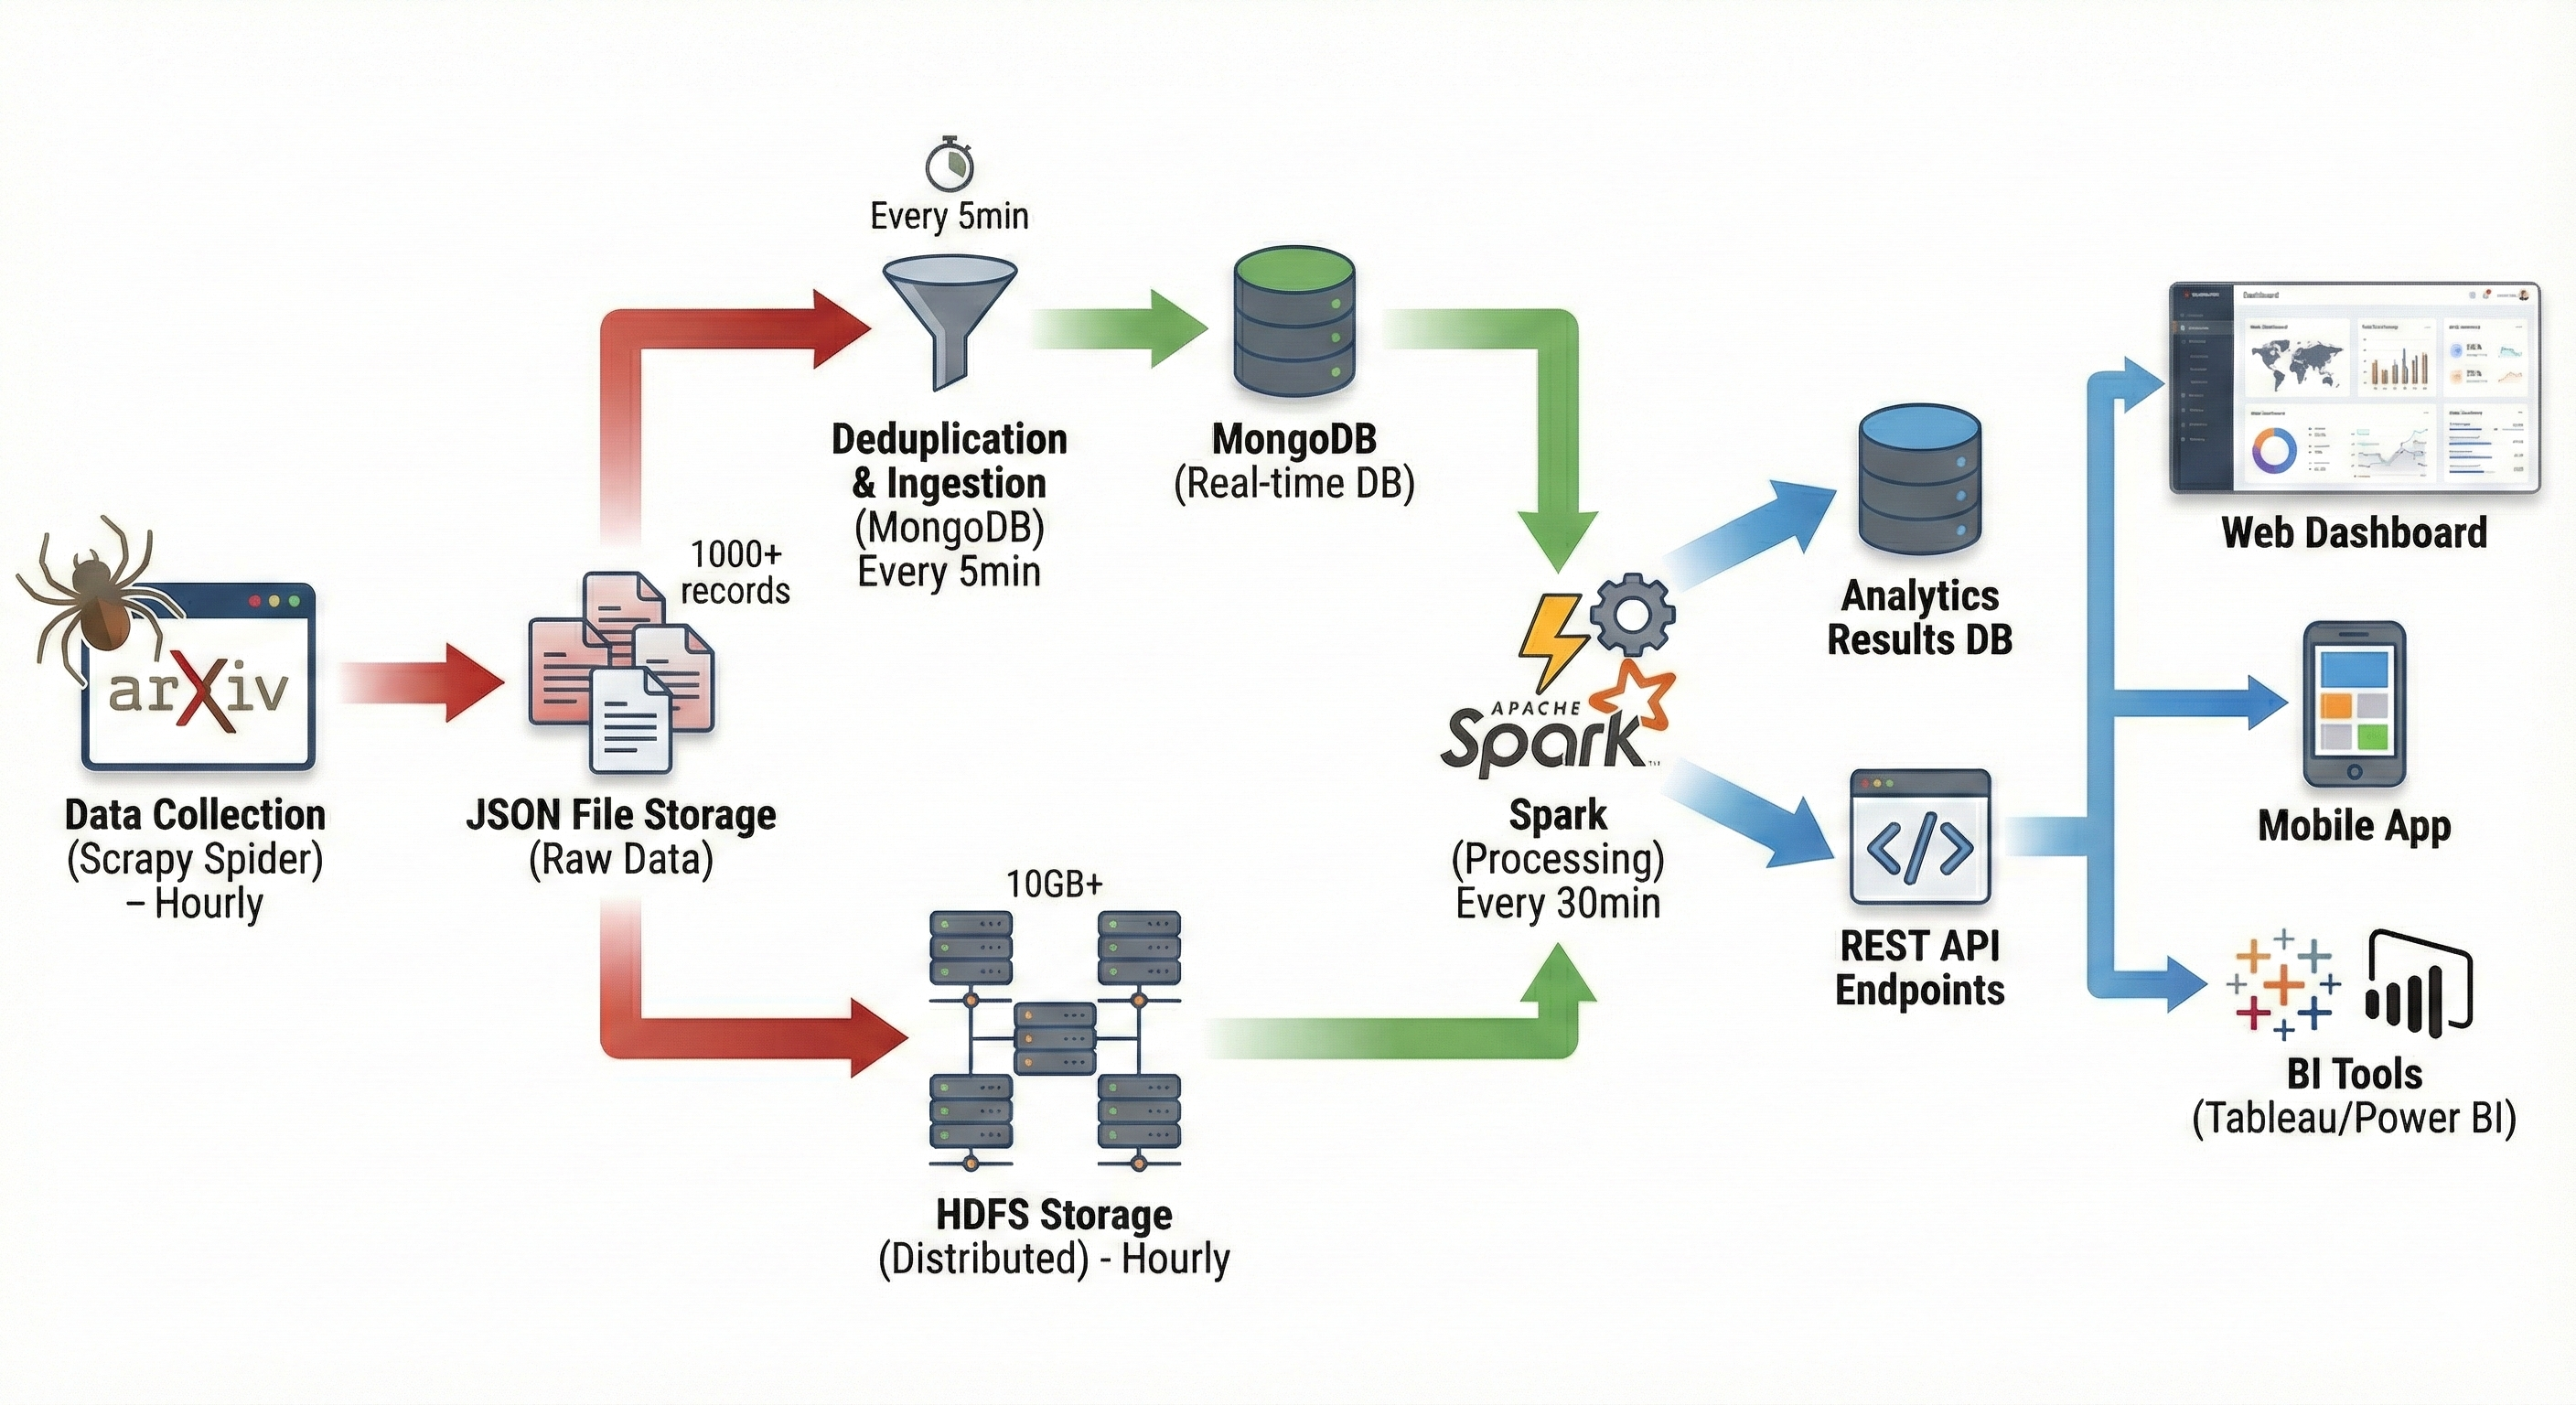
\includegraphics[width=0.9\textwidth]{images/System-Architecture-Diagram.png}
    \caption{System Architecture Overview}
    \label{fig:architecture}
\end{figure}

\subsection{Architectural Layers}

\subsubsection{Layer 1: Data Collection Layer}

The data collection layer is responsible for automated web scraping of research papers from arXiv.org. Key components:

\begin{itemize}
    \item \textbf{Scrapy Spider:} Crawls arXiv.org with configurable search parameters
    \item \textbf{Scheduling Mechanism:} Executes scraping jobs every hour
    \item \textbf{Data Extraction:} Parses HTML and extracts structured information
    \item \textbf{Output Generation:} Produces JSON files with timestamped filenames
\end{itemize}

\subsubsection{Layer 2: Storage Layer}

The storage layer implements a hybrid approach combining NoSQL and distributed file systems:

\begin{itemize}
    \item \textbf{MongoDB:} Stores structured data for fast queries and real-time access
    \item \textbf{Hadoop HDFS:} Archives data for long-term storage and batch processing
    \item \textbf{Data Storage Service:} Monitors new files and stores them in MongoDB
    \item \textbf{HDFS Storage Service:} Archives data to HDFS for distributed processing
    \item \textbf{Deduplication Logic:} Prevents duplicate entries based on title and authors
\end{itemize}

\subsubsection{Layer 3: Processing Layer}

The processing layer performs distributed analytics using Apache Spark:

\begin{itemize}
    \item \textbf{Spark Master:} Coordinates distributed computations
    \item \textbf{Spark Workers:} Execute parallel processing tasks
    \item \textbf{Analysis Jobs:} Generate statistics, trends, and aggregations
    \item \textbf{Scheduling:} Runs analytics every 30 minutes
\end{itemize}

\subsubsection{Layer 4: API Layer}

The API layer exposes data and analytics through RESTful endpoints:

\begin{itemize}
    \item \textbf{Flask API:} Provides basic CRUD operations
    \item \textbf{Smart Router:} Implements intelligent query routing
    \item \textbf{Routing Logic:} Selects optimal data source based on query complexity
    \item \textbf{Response Formatting:} Returns JSON responses with metadata
\end{itemize}

\subsubsection{Layer 5: Presentation Layer}

The presentation layer provides user interfaces for data exploration:

\begin{itemize}
    \item \textbf{Web Dashboard:} Interactive HTML5 application
    \item \textbf{Search Interface:} Text search and advanced filtering
    \item \textbf{Visualizations:} Charts, graphs, and geographic maps
    \item \textbf{Real-time Updates:} Dynamic content loading via AJAX
\end{itemize}

\subsection{Data Flow Architecture}

\begin{figure}[H]
    \centering
    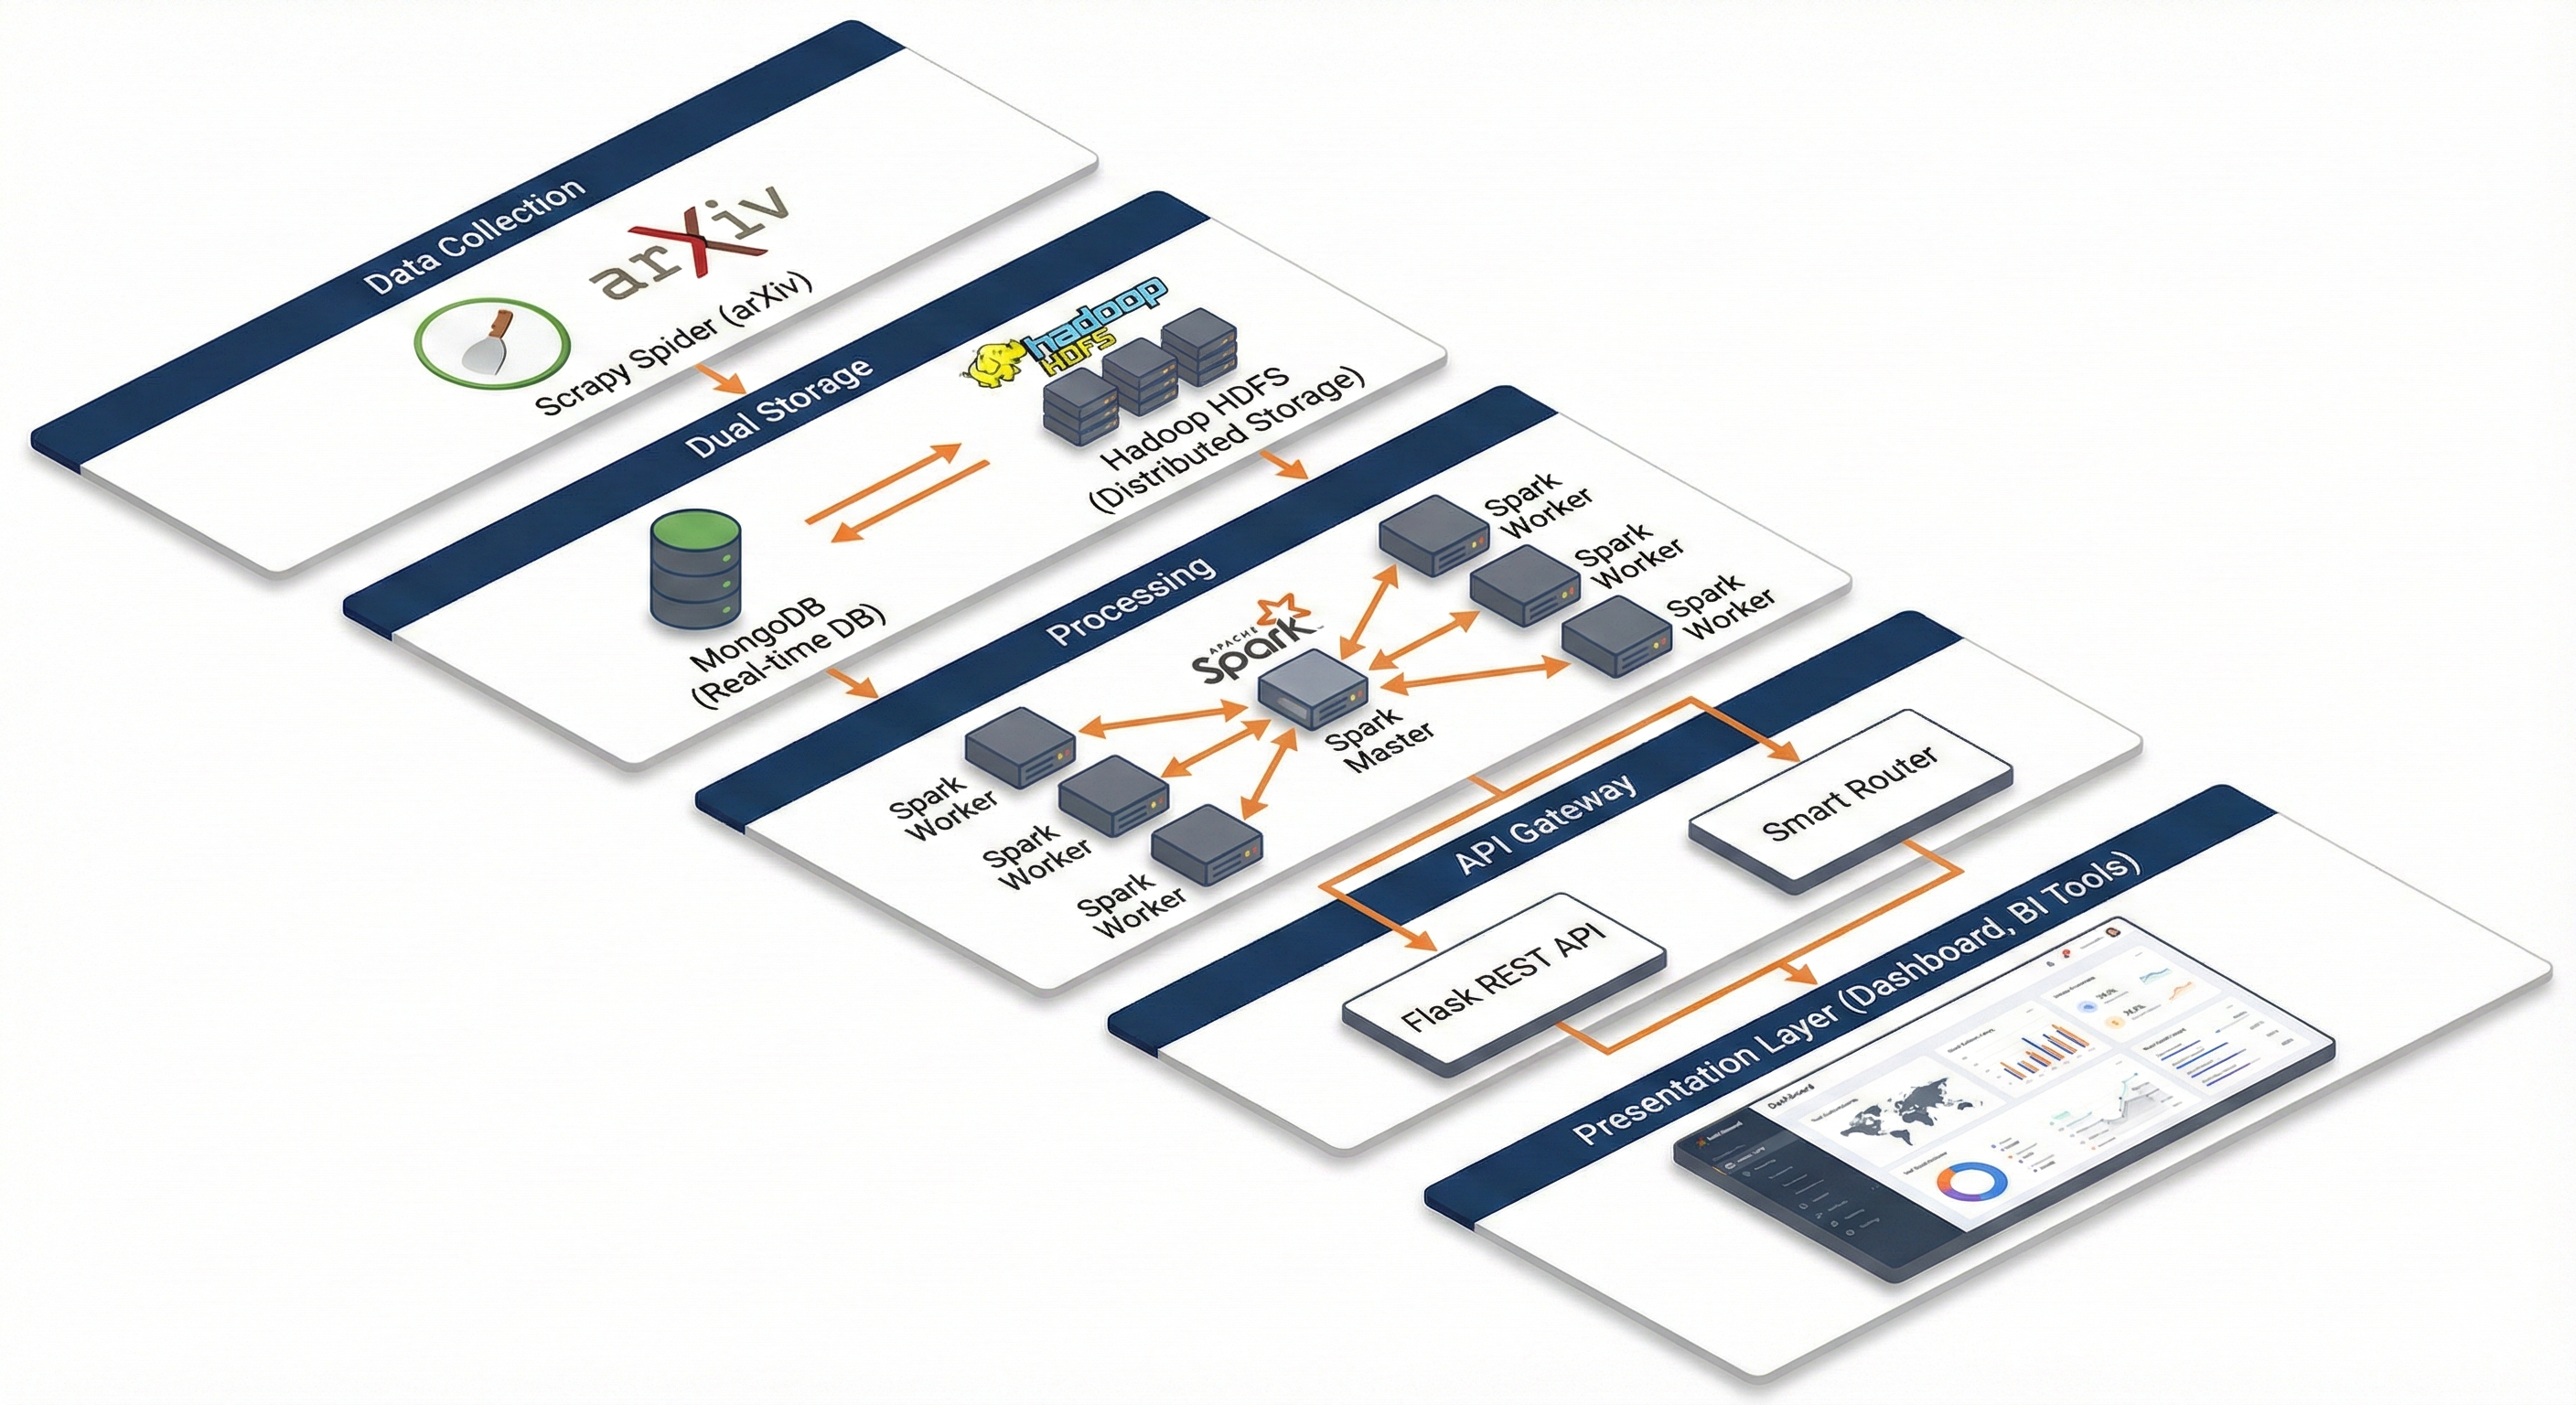
\includegraphics[width=0.9\textwidth]{images/End-to-End-Data-Flow-Pipeline.png}
    \caption{End-to-End Data Flow Pipeline}
    \label{fig:dataflow}
\end{figure}

The data flow follows these stages:

\begin{enumerate}
    \item \textbf{Extraction:} Scrapy spider extracts data from arXiv.org
    \item \textbf{Serialization:} Data is serialized to JSON format
    \item \textbf{Storage:} JSON files are stored in the /data directory
    \item \textbf{Ingestion:} Storage service reads new files every 5 minutes
    \item \textbf{Validation:} Data is validated and deduplicated
    \item \textbf{Persistence:} Valid data is stored in MongoDB and HDFS
    \item \textbf{Processing:} Spark reads data and performs analytics
    \item \textbf{Aggregation:} Results are aggregated and stored
    \item \textbf{Serving:} API exposes data to clients
    \item \textbf{Visualization:} Dashboard displays interactive visualizations
\end{enumerate}

\subsection{Design Patterns}

\subsubsection{Microservices Pattern}

Each component is designed as an independent microservice:

\begin{itemize}
    \item Scrapy service for data collection
    \item MongoDB service for NoSQL storage
    \item Hadoop services for distributed storage
    \item Spark services for distributed processing
    \item API services for data access
    \item Dashboard service for user interface
\end{itemize}

\subsubsection{Repository Pattern}

Data access is abstracted through repository interfaces, separating business logic from data access logic.

\subsubsection{Strategy Pattern}

The smart router implements the strategy pattern to select between MongoDB and HDFS based on query characteristics.

\subsubsection{Observer Pattern}

The data storage service observes the /data directory for new files and triggers processing workflows.

\subsection{Scalability Considerations}

The architecture supports both vertical and horizontal scaling:

\begin{itemize}
    \item \textbf{Horizontal Scaling:} Add more Spark workers, MongoDB replicas, or HDFS data nodes
    \item \textbf{Vertical Scaling:} Increase resources (CPU, RAM) for individual services
    \item \textbf{Load Balancing:} Distribute requests across multiple API instances
    \item \textbf{Caching:} Implement Redis for frequently accessed data
\end{itemize}

\newpage

\section{Technology Stack and Tools}

\subsection{Programming Languages}

\subsubsection{Python 3.8+}

Python serves as the primary programming language for:

\begin{itemize}
    \item Web scraping with Scrapy
    \item Data processing with PySpark
    \item API development with Flask
    \item Automation scripts
\end{itemize}

Advantages: Rich ecosystem, extensive libraries, readability, and strong Big Data support.

\subsubsection{JavaScript (ES6+)}

JavaScript powers the frontend dashboard:

\begin{itemize}
    \item DOM manipulation
    \item AJAX requests
    \item Interactive visualizations
    \item Event handling
\end{itemize}

\subsubsection{HTML5 and CSS3}

Modern web standards for responsive user interfaces.

\subsection{Data Collection}

\subsubsection{Apache Scrapy 2.x}

Scrapy is a powerful web scraping framework featuring:

\begin{itemize}
    \item Asynchronous request handling
    \item Built-in selectors (XPath, CSS)
    \item Item pipelines for data processing
    \item Middleware for request/response processing
    \item Automatic throttling and politeness
\end{itemize}

Configuration:
\begin{lstlisting}[language=Python]
CLOSESPIDER_ITEMCOUNT = 1000
DOWNLOAD_DELAY = 2.5
CONCURRENT_REQUESTS = 16
\end{lstlisting}

\subsection{Data Storage}

\subsubsection{MongoDB 6.x}

MongoDB provides flexible document storage:

\begin{itemize}
    \item Document-oriented data model
    \item Rich query language
    \item Aggregation framework
    \item Indexing for performance
    \item Replication for high availability
\end{itemize}

Database structure:
\begin{itemize}
    \item Database: \texttt{dynamic\_data\_db}
    \item Collection: \texttt{raw\_data}
    \item Indexes: title, authors, year, keyword, country
\end{itemize}

\subsubsection{Hadoop HDFS 3.x}

HDFS provides distributed file storage:

\begin{itemize}
    \item NameNode: Manages metadata and namespace
    \item DataNode: Stores actual data blocks
    \item Replication factor: 3 (default)
    \item Block size: 128 MB
\end{itemize}

\subsection{Data Processing}

\subsubsection{Apache Spark 3.x}

Spark enables distributed data processing:

\begin{itemize}
    \item Spark Core: Basic functionality and RDDs
    \item Spark SQL: Structured data processing
    \item DataFrame API: High-level data manipulation
    \item Catalyst optimizer: Query optimization
\end{itemize}

Cluster configuration:
\begin{itemize}
    \item 1 Master node (coordinator)
    \item 1+ Worker nodes (executors)
    \item Memory: 1GB per worker
    \item Cores: 1 core per worker
\end{itemize}

\subsection{API Development}

\subsubsection{Flask 2.x}

Flask is a lightweight web framework:

\begin{itemize}
    \item RESTful routing
    \item Request/response handling
    \item JSON serialization
    \item CORS support via Flask-CORS
\end{itemize}

\subsubsection{PyMongo}

Python driver for MongoDB:

\begin{itemize}
    \item Connection pooling
    \item Query building
    \item Cursor management
    \item Aggregation pipeline support
\end{itemize}

\subsection{Frontend Technologies}

\subsubsection{Leaflet.js}

Interactive mapping library:

\begin{itemize}
    \item Tile layer management
    \item Marker clustering
    \item Popup windows
    \item Zoom controls
\end{itemize}

\subsubsection{OpenStreetMap}

Open-source map tiles for geographic visualization.

\subsection{Containerization}

\subsubsection{Docker 20.x}

Container platform for application packaging:

\begin{itemize}
    \item Dockerfile for image definition
    \item Layer caching for efficiency
    \item Volume mounting for data persistence
    \item Network isolation
\end{itemize}

\subsubsection{Docker Compose 2.x}

Multi-container orchestration:

\begin{itemize}
    \item Service definition in YAML
    \item Dependency management
    \item Network creation
    \item Volume management
\end{itemize}

Total services: 11 containers
\begin{itemize}
    \item mongo
    \item hadoop-namenode
    \item hadoop-datanode
    \item spark-master
    \item spark-worker
    \item scrapy
    \item data-storage
    \item hdfs-storage
    \item spark-analyzer
    \item smart-router
    \item dashboard
\end{itemize}

\subsection{Development Tools}

\begin{itemize}
    \item \textbf{Git:} Version control
    \item \textbf{GitHub:} Code hosting and collaboration
    \item \textbf{VS Code:} Integrated development environment
    \item \textbf{Postman:} API testing
    \item \textbf{MongoDB Compass:} Database GUI
\end{itemize}

\newpage
